На основе анализа теоретических аспектов военно-политических игр, возможностей и ограничений современных языковых моделей, а также существующих подходов к автоматизации геймплея, можно сформулировать комплексную задачу разработки мультиагентной текстовой стратегической игры на основе оркестрируемых языковых моделей. Данная глава детализирует функциональные и нефункциональные требования к разрабатываемой системе, описывает ключевых акторов и сценарии взаимодействия с системой, а также представляет архитектурные решения, обеспечивающие эффективное функционирование игры. Особое внимание уделяется специфике интеграции языковых моделей для автоматизации роли вердера с учетом выявленных ограничений и оптимальных методов их преодоления. Представленные в данной главе решения служат основой для последующей разработки как первичного прототипа системы, так и её улучшенной версии.
\subsection{Анализ требований пользователей}

Для разработки эффективной мультиагентной текстовой стратегической игры на основе оркестрируемых языковых моделей критически важно понимание ожиданий, предпочтений и потребностей целевой аудитории. В рамках исследования было проведено детальное интервьюирование потенциальных пользователей (подробные результаты представлены в Приложении~\ref{appendix:1}), что позволило выявить ключевые требования и сформировать целостное представление о желаемых характеристиках системы.

\subsubsection{Платформа и пользовательский интерфейс}

Анализ предпочтений пользователей относительно платформы проведения игры показал явное преобладание Telegram как предпочтительной платформы. Около 50\% респондентов однозначно высказались за использование данного мессенджера, аргументируя свой выбор удобством разметки, лучшей системой уведомлений и более интуитивным интерфейсом. Примерно 30\% опрошенных не выразили явных предпочтений между различными платформами, в то время как меньшинство (около 20\%) предпочли бы использование ВКонтакте.

Исходя из этих данных, Telegram определяется как основная платформа для разработки игрового интерфейса, с возможным последующим расширением на другие платформы.

\subsubsection{Монетизация и игровой темп}

Вопрос монетизации игры выявил значительную дифференциацию в готовности пользователей оплачивать игровые услуги:

\begin{itemize}
    \item Около 40\% опрошенных выразили готовность платить за игровые услуги в диапазоне от 300 до 2000 рублей в месяц, с преобладанием ценового диапазона 300-500 рублей.

    \item Оставшиеся 60\% предпочли бы бесплатный формат, с возможностью единоразовых пожертвований.
\end{itemize}

Анализ предпочтений относительно темпа игры выявил корреляцию между готовностью платить и желаемой частотой получения вердиктов. Пользователи, готовые платить большие суммы, ожидают более высокого темпа игры (до нескольких вердиктов в день), в то время как сторонники бесплатного формата удовлетворены более медленным темпом (около одного вердикта в день или реже).

На основе этих данных рекомендуется разработка многоуровневой системы монетизации:

\begin{enumerate}
    \item Бесплатный базовый уровень с ограниченным количеством вердиктов (1 в день или реже).

    \item Средний платный уровень (300-500 рублей в месяц) с умеренным темпом игры (2-3 верда в день).

    \item Премиум-уровень (1000-2000 рублей в месяц) с высоким темпом игры и дополнительными возможностями.
\end{enumerate}

\subsubsection{Игровые механики и особенности}

\paragraph{Отношение к элементам случайности}

Анализ отношения игроков к использованию случайности в игровом процессе выявил следующую картину:

\begin{itemize}
    \item Около 60\% респондентов выразили положительное отношение к включению элементов случайности в игровой процесс, предпочитая баланс между предопределенными результатами и случайными событиями. Многие указали на желательное соотношение 7:3, где 70\% результатов определяются действиями игрока, а 30\% — случайными факторами.

    \item Примерно 30\% выразили нейтральное отношение, не имея сильных предпочтений.

    \item Лишь 10\% участников высказались против использования случайности в игре, допуская её только в редких случаях (например, катаклизмы или чрезвычайные события).
\end{itemize}

Учитывая эти предпочтения, рекомендуется реализация настраиваемой системы случайности с возможностью регулирования её влияния на игровой процесс (параметр temperature в запросах к языковой модели) и обеспечения прозрачности в определении результатов действий.

\paragraph{Боевая система}

Предпочтения относительно боевой системы демонстрируют разнообразие подходов:

\begin{itemize}
    \item Большинство игроков предпочитают стратегический уровень принятия решений, где они определяют общие направления действий, а не управляют каждым юнитом напрямую.

    \item Некоторые игроки выразили желание иметь возможность выбора между детальным управлением и стратегическими приказами в зависимости от ситуации.

    \item Отдельные участники высказались за использование систем на основе кубиков (по аналогии с D\&D) для определения результатов сражений.
\end{itemize}

Оптимальным решением представляется создание гибкой боевой системы, позволяющей игрокам выбирать уровень детализации своего участия в военных действиях, с сохранением акцента на стратегических решениях и их нарративной интерпретации.

\paragraph{Визуализация и мультимедиа}

Относительно визуальных элементов игры выявлены следующие предпочтения:

\begin{itemize}
    \item Около 50\% респондентов проявили интерес к автоматической генерации изображений, иллюстрирующих значимые события и результаты действий.

    \item Большинство игроков (около 70\%) положительно отнеслись к использованию графиков и диаграмм для отображения экономических показателей, военной мощи и других количественных характеристик.

    \item Примерно 30\% опрошенных выразили интерес к функции расшифровки голосовых сообщений для упрощения коммуникации.
\end{itemize}

Рекомендуется внедрение опциональных визуальных элементов, дополняющих основной текстовый формат игры, с акцентом на информативности и эстетической ценности.

\subsubsection{Отношение к использованию языковых моделей}

Анализ отношения игроков к применению языковых моделей в роли вердера показал следующие результаты:

\begin{itemize}
    \item Около 40\% респондентов выразили положительное отношение к использованию ИИ для автоматизации вердинга, отмечая потенциальные преимущества в скорости и доступности.

    \item Примерно 30\% заняли нейтральную позицию, не видя принципиальных препятствий, но выражая определенные опасения относительно качества и последовательности генерируемого контента.

    \item Около 30\% высказали негативное отношение, опасаясь потери человеческого творческого элемента и уникального стиля, присущего человеку-вердеру.
\end{itemize}

Многие участники, независимо от общего отношения, выразили беспокойство относительно способности языковых моделей сохранять контекст игры, учитывать специфику игрового мира и обеспечивать последовательность нарратива. Часто высказывалось пожелание сохранить роль человека-администратора для надзора и корректировки действий ИИ.

\subsubsection{Коммуникационные предпочтения}

В вопросе организации коммуникации между игроками мнения разделились:

\begin{itemize}
    \item Около 60\% предпочитают общение через игрового бота, что обеспечивает сохранение всех коммуникаций в общем контексте игры и потенциально увеличивает иммерсивность.

    \item Примерно 40\% высказались за использование традиционных каналов коммуникации (групповые чаты, личные сообщения), обеспечивающих более непосредственное взаимодействие.
\end{itemize}

Некоторые игроки также выразили заинтересованность в механизмах, обеспечивающих анонимность коммуникации для предотвращения "метаигры" — ситуаций, когда личные отношения между игроками влияют на игровой процесс.

\subsubsection{Ключевые выводы и приоритетные требования}

На основе проведенного анализа можно сформулировать следующие ключевые требования к разрабатываемой системе:

\begin{enumerate}
    \item Реализация интерфейса на платформе Telegram с интуитивно понятной навигацией и системой уведомлений.

    \item Создание многоуровневой системы монетизации, обеспечивающей различные темпы игры в зависимости от выбранного тарифа.

    \item Внедрение настраиваемых элементов случайности с преобладанием детерминированных результатов, зависящих от действий игрока.

    \item Разработка гибкой боевой системы с акцентом на стратегическом уровне принятия решений.

    \item Интеграция визуальных элементов (графики, диаграммы, генерируемые изображения) как дополнение к основному текстовому контенту.

    \item Обеспечение механизмов сохранения контекста и последовательности игрового мира при использовании языковых моделей.

    \item Сохранение роли человека-администратора для надзора и корректировки автоматически генерируемого контента.

    \item Создание интегрированной системы коммуникации с возможностью выбора между игровыми и внеигровыми каналами общения.

    \item Разработка механизмов для баланса между автоматизацией и сохранением уникального игрового опыта.
\end{enumerate}

Эти требования являются фундаментом для дальнейшей разработки функциональных и нефункциональных спецификаций системы и определяют основные направления проектирования архитектуры мультиагентной системы для автоматизации ВПИ.

\subsection{Функциональные требования к системе}

На основе проведенного анализа требований пользователей и с учетом специфики военно-политических игр и возможностей современных языковых моделей, можно сформулировать следующие функциональные требования к разрабатываемой мультиагентной системе.

\subsubsection{Основные игровые функции}

\begin{enumerate}[label=FR\arabic*.]
    \item \textbf{Обработка приказов игроков:} Система должна принимать, обрабатывать и интерпретировать текстовые приказы игроков, направленные на управление виртуальным государством.

    \item \textbf{Генерация вердиктов:} Система должна генерировать содержательные, логически согласованные текстовые описания результатов выполнения приказов игроков с учетом текущего состояния игрового мира и механик игры.

    \item \textbf{Управление игровым миром:} Система должна поддерживать и обновлять состояние игрового мира, включая экономические показатели, военный потенциал, демографические характеристики и дипломатические отношения между государствами.

    \item \textbf{Симуляция проектов:} Система должна моделировать выполнение долгосрочных проектов, инициированных игроками (строительство инфраструктуры, разработка технологий и т.д.), с учетом имеющихся ресурсов и временных рамок.

    \item \textbf{Обработка военных действий:} Система должна моделировать сражения и военные кампании на основе приказов игроков, с учетом численности войск, их качества, тактических решений и географических условий.

    \item \textbf{Управление дипломатией:} Система должна обрабатывать дипломатические взаимодействия между государствами, включая заключение договоров, формирование альянсов, объявление войн и ведение переговоров.

    \item \textbf{Генерация игровых событий:} Система должна периодически создавать внутриигровые события (природные катаклизмы, восстания, культурные явления и т.д.) для обогащения игрового нарратива и создания новых вызовов для игроков.
\end{enumerate}

\subsubsection{Учетные записи и управление игрой}

\begin{enumerate}[label=FR\arabic*., resume]
    \item \textbf{Регистрация и аутентификация:} Система должна обеспечивать регистрацию новых игроков, аутентификацию существующих пользователей и управление игровыми сессиями.

    \item \textbf{Создание и настройка государства:} Система должна позволять игрокам создавать и настраивать виртуальные государства, определяя их географические, политические и экономические характеристики в соответствии с правилами игры.

    \item \textbf{Управление игровыми сессиями:} Система должна поддерживать механизмы создания новых игровых сессий, присоединения игроков к существующим сессиям и завершения игр.

    \item \textbf{Настройка игровых параметров:} Система должна позволять администраторам и, в определенных пределах, игрокам настраивать параметры игры, такие как скорость игрового времени, степень случайности и тематические ограничения.

    \item \textbf{Учет игровой активности:} Система должна отслеживать активность игроков для применения правил отсутствия (AFK) и автоматического управления неактивными государствами.
\end{enumerate}

\subsubsection{Мультиагентная обработка приказов}

\begin{enumerate}[label=FR\arabic*., resume]
    \item \textbf{Валидация приказов:} Система должна проверять соответствие приказов игроков установленным правилам, текущему технологическому уровню и имеющимся ресурсам.

    \item \textbf{Классификация приказов:} Система должна определять тип и сферу действия приказа (экономический, военный, дипломатический и т.д.) для его соответствующей обработки.

    \item \textbf{Проверка на соответствие эпохе:} Система должна оценивать соответствие приказов историческому или тематическому контексту игрового мира, предотвращая анахронизмы и нарушения жанровой целостности.

    \item \textbf{Оценка влияния на игровые параметры:} Система должна анализировать потенциальное влияние приказов на различные параметры государства (экономика, лояльность населения, военная мощь) и генерировать соответствующие изменения.

    \item \textbf{Разрешение конфликтов:} Система должна обеспечивать механизмы разрешения конфликтующих приказов разных игроков, особенно в ситуациях прямого противостояния.
\end{enumerate}

\subsubsection{Коммуникационные функции}

\begin{enumerate}[label=FR\arabic*., resume]
    \item \textbf{Внутриигровая переписка:} Система должна обеспечивать возможность обмена сообщениями между игроками с имитацией дипломатической переписки и сохранением в общем контексте игры.

    \item \textbf{Публичные объявления:} Система должна поддерживать функционал для публикации официальных заявлений государств, видимых всем участникам игры.

    \item \textbf{Секретные коммуникации:} Система должна обеспечивать возможность конфиденциальных переговоров между выбранными участниками, с опциональной возможностью перехвата при определенных игровых условиях.

    \item \textbf{Новостные сводки:} Система должна генерировать периодические новостные отчеты о ключевых событиях в игровом мире, доступные всем игрокам.
\end{enumerate}

\subsubsection{Визуализация и пользовательский интерфейс}

\begin{enumerate}[label=FR\arabic*., resume]
    \item \textbf{Игровая карта:} Система должна предоставлять интерактивную карту игрового мира с отображением государственных границ, ресурсов, военных подразделений и других релевантных объектов.

    \item \textbf{Экономические графики:} Система должна генерировать и отображать графики экономического развития государств, включая ключевые показатели (ВВП, уровень жизни, производственные мощности).

    \item \textbf{Военная статистика:} Система должна предоставлять визуализацию военного потенциала государств, включая численность войск, их качество и распределение.

    \item \textbf{Генерация изображений:} Система должна создавать иллюстрации к значимым событиям и результатам действий с использованием технологий генерации изображений.

    \item \textbf{Исторический журнал:} Система должна поддерживать хронологическую запись всех значимых игровых событий с возможностью просмотра и поиска.
\end{enumerate}

\subsubsection{Управление контекстом и состоянием игры}

\begin{enumerate}[label=FR\arabic*., resume]
    \item \textbf{Сохранение состояния игрового мира:} Система должна сохранять и обновлять полное состояние игрового мира, включая все государства, отношения между ними и глобальные параметры.

    \item \textbf{Резюмирование истории:} Система должна создавать и обновлять сжатые резюме исторического развития государств и мира в целом для эффективного использования ограниченного контекстного окна языковых моделей.

    \item \textbf{Извлечение релевантной информации:} Система должна эффективно извлекать информацию, релевантную для обработки конкретного приказа, из общего хранилища данных об игровом мире.

    \item \textbf{Обнаружение и коррекция несоответствий:} Система должна идентифицировать потенциальные логические несоответствия и противоречия в генерируемом контенте и предпринимать меры для их устранения.
\end{enumerate}

\subsubsection{Административные функции}

\begin{enumerate}[label=FR\arabic*., resume]
    \item \textbf{Мониторинг игрового процесса:} Система должна предоставлять инструменты для отслеживания общего состояния игры, активности игроков и потенциальных проблем.

    \item \textbf{Ручное вмешательство:} Система должна поддерживать механизмы для ручной корректировки автоматически генерируемого контента, разрешения спорных ситуаций и внесения изменений в игровой мир.

    \item \textbf{Управление параметрами ИИ:} Система должна предоставлять интерфейс для настройки параметров языковых моделей (температуры, предвзятости, максимальной длины ответа) для оптимизации качества генерируемого контента.

    \item \textbf{Журналирование и аудит:} Система должна вести детальный журнал всех значимых действий и операций для анализа, отладки и разрешения потенциальных споров.
\end{enumerate}

\subsubsection{Расширенные функции и монетизация}

\begin{enumerate}[label=FR\arabic*., resume]
    \item \textbf{Управление тарифными планами:} Система должна поддерживать различные уровни доступа с соответствующими ограничениями и возможностями в зависимости от выбранного игроком тарифа.

    \item \textbf{Обработка платежей:} Система должна обеспечивать безопасную обработку платежей для платных тарифов и учет финансовых транзакций.

    \item \textbf{Система достижений:} Система должна отслеживать игровые достижения пользователей и предоставлять соответствующие награды или признание.

    \item \textbf{Аналитика пользовательского опыта:} Система должна собирать и анализировать данные о пользовательском опыте для выявления проблемных аспектов и возможностей улучшения.

    \item \textbf{Расширенные инструменты для премиум-пользователей:} Система должна предоставлять дополнительные инструменты анализа, планирования и визуализации для пользователей премиум-тарифов.
\end{enumerate}

\subsubsection{Безопасность и этические аспекты}

\begin{enumerate}[label=FR\arabic*., resume]
    \item \textbf{Фильтрация неприемлемого контента:} Система должна выявлять и блокировать потенциально оскорбительный, вредоносный или неприемлемый контент в приказах игроков и коммуникациях.

    \item \textbf{Обеспечение конфиденциальности:} Система должна защищать конфиденциальность игровых взаимодействий и личных данных пользователей.

    \item \textbf{Предотвращение злоупотреблений:} Система должна включать механизмы для предотвращения злоупотреблений игровыми механиками и эксплуатации уязвимостей.

    \item \textbf{Соблюдение тематических ограничений:} Система должна обеспечивать соблюдение установленных тематических и жанровых ограничений игрового мира.
\end{enumerate}

Перечисленные функциональные требования формируют основу для проектирования архитектуры системы и разработки конкретных компонентов мультиагентной текстовой стратегической игры. Они будут дополнены и конкретизированы в процессе более детального проектирования отдельных модулей системы.

\subsection{Нефункциональные требования}

Нефункциональные требования определяют качественные характеристики и ограничения системы, которые напрямую не связаны с конкретными функциями, но критически важны для обеспечения удовлетворительного пользовательского опыта, производительности, безопасности и других аспектов работы мультиагентной текстовой стратегической игры.

\subsubsection{Производительность и отзывчивость}

\begin{enumerate}[label=NFR\arabic*.]
    \item \textbf{Время обработки приказов:} Система должна обрабатывать стандартные приказы и генерировать вердикты в течение не более 2 минут для 90\% запросов. Для особо сложных приказов, требующих моделирования комплексных сценариев, допустимое время обработки может быть увеличено до 5 минут.

    \item \textbf{Поддержка одновременных пользователей:} Система должна обеспечивать стабильную работу с одновременным обслуживанием не менее 100 активных игроков в рамках одной игровой сессии без заметного ухудшения производительности.

    \item \textbf{Отзывчивость интерфейса:} Время отклика пользовательского интерфейса на стандартные действия (навигация, просмотр информации) не должно превышать 1 секунды в 95\% случаев.

    \item \textbf{Обработка сообщений:} Обмен сообщениями между игроками должен происходить практически в реальном времени, с задержкой не более 2 секунд при нормальных условиях работы сети.
\end{enumerate}

\subsubsection{Масштабируемость и доступность}

\begin{enumerate}[label=NFR\arabic*., resume]
    \item \textbf{Горизонтальная масштабируемость:} Архитектура системы должна поддерживать горизонтальное масштабирование для обслуживания растущего числа пользователей без необходимости фундаментальной реструктуризации.

    \item \textbf{Доступность системы:} Система должна быть доступна не менее 99.5\% времени, исключая запланированные периоды технического обслуживания.

    \item \textbf{Устойчивость к сбоям:} Система должна сохранять работоспособность в случае частичных сбоев инфраструктуры или отдельных компонентов, обеспечивая деградацию функциональности вместо полного отказа.

    \item \textbf{Период восстановления:} В случае критического сбоя, система должна восстанавливаться в течение не более 2 часов с минимальной потерей данных (целевая точка восстановления — не более 10 минут потерянных транзакций).
\end{enumerate}

\subsubsection{Надежность и целостность данных}

\begin{enumerate}[label=NFR\arabic*., resume]
    \item \textbf{Сохранение игрового состояния:} Система должна регулярно сохранять полное состояние игрового мира, обеспечивая возможность восстановления в случае сбоя с минимальной потерей прогресса.

    \item \textbf{Согласованность данных:} Система должна поддерживать согласованность всех взаимозависимых данных, особенно в контексте параллельных действий нескольких игроков, затрагивающих одни и те же аспекты игрового мира.

    \item \textbf{Достоверность генерации:} Система должна минимизировать возникновение "галлюцинаций" языковых моделей, обеспечивая фактическую точность в отношении установленных аспектов игрового мира с точностью не менее 95\%.

    \item \textbf{Обнаружение аномалий:} Система должна включать механизмы обнаружения аномальных игровых состояний, нелогичных последовательностей событий или потенциальных противоречий в нарративе.
\end{enumerate}

\subsubsection{Безопасность и конфиденциальность}

\begin{enumerate}[label=NFR\arabic*., resume]
    \item \textbf{Защита пользовательских данных:} Система должна обеспечивать защиту личных данных пользователей в соответствии с применимыми нормативными требованиями (GDPR, 152-ФЗ и другие).

    \item \textbf{Предотвращение несанкционированного доступа:} Система должна включать многоуровневые механизмы аутентификации и авторизации для предотвращения несанкционированного доступа к административным функциям и конфиденциальным данным.

    \item \textbf{Изоляция игровых сессий:} Система должна обеспечивать логическую изоляцию различных игровых сессий для предотвращения перекрестного влияния или утечки информации.

    \item \textbf{Безопасность API:} Все внешние интерфейсы API должны быть защищены соответствующими механизмами аутентификации и шифрования, с ограничением частоты запросов для предотвращения DoS-атак.

    \item \textbf{Модерация контента:} Система должна обеспечивать эффективную модерацию пользовательского контента для предотвращения распространения вредоносного, оскорбительного или незаконного материала.
\end{enumerate}

\subsubsection{Удобство использования и доступность}

\begin{enumerate}[label=NFR\arabic*., resume]
    \item \textbf{Интуитивный интерфейс:} Интерфейс системы должен быть интуитивно понятным, позволяя новым пользователям освоить основные функции без обширного обучения (не более 30 минут для базового освоения).

    \item \textbf{Документация и обучение:} Система должна включать исчерпывающую документацию и обучающие материалы, охватывающие все аспекты игрового процесса и интерфейса.

    \item \textbf{Адаптивный дизайн:} Интерфейс должен корректно отображаться и функционировать на различных устройствах и размерах экрана (мобильные телефоны, планшеты, настольные компьютеры).
\end{enumerate}

\subsubsection{Технологические требования и совместимость}

\begin{enumerate}[label=NFR\arabic*., resume]
    \item \textbf{Кроссплатформенность:} Клиентская часть системы должна функционировать на основных платформах (iOS, Android, Windows, macOS, Linux) через веб-интерфейс или нативные клиенты.

    \item \textbf{Интеграция с мессенджерами:} Система должна обеспечивать интеграцию с популярными мессенджерами, в первую очередь с Telegram, для обеспечения удобного доступа к игровым функциям.

    \item \textbf{Модульная архитектура:} Система должна иметь модульную архитектуру, позволяющую независимое развитие и обновление отдельных компонентов без нарушения функциональности всей системы.

    \item \textbf{API для расширений:} Система должна предоставлять документированные API для потенциальной разработки сторонних расширений и интеграций.

    \item \textbf{Совместимость с языковыми моделями:} Система должна поддерживать взаимодействие с различными языковыми моделями (GPT, Claude, Llama и другие) через унифицированный интерфейс для обеспечения гибкости и устойчивости к изменениям в экосистеме ИИ.
\end{enumerate}

\subsubsection{Эффективность и оптимизация ресурсов}

\begin{enumerate}[label=NFR\arabic*., resume]
    \item \textbf{Оптимизация запросов к LLM:} Система должна минимизировать количество и объем запросов к языковым моделям через эффективное управление контекстом, кэширование и другие механизмы оптимизации.

    \item \textbf{Эффективное хранение данных:} Схема хранения игровых данных должна быть оптимизирована для минимизации избыточности и обеспечения эффективного доступа к часто запрашиваемой информации.

    \item \textbf{Энергоэффективность:} Система должна быть спроектирована с учетом энергоэффективности, особенно в контексте вычислительно интенсивных операций, связанных с языковыми моделями.

    \item \textbf{Экономическая эффективность:} Операционные расходы на поддержание системы (включая API-вызовы к языковым моделям) должны быть оптимизированы для обеспечения экономической устойчивости проекта.
\end{enumerate}

\subsubsection{Обслуживаемость и развитие}

\begin{enumerate}[label=NFR\arabic*., resume]
    \item \textbf{Мониторинг и логирование:} Система должна включать комплексные механизмы мониторинга и логирования для облегчения диагностики проблем и анализа производительности.

    \item \textbf{Обновляемость:} Архитектура системы должна поддерживать регулярные обновления компонентов без значительных прерываний в обслуживании (целевое время простоя для обновлений — не более 2 часов в месяц).

    \item \textbf{Обратная совместимость:} Обновления системы должны сохранять обратную совместимость с существующими данными и интерфейсами, минимизируя необходимость миграции или адаптации для пользователей.

    \item \textbf{Документация кода:} Исходный код системы должен быть хорошо документирован для облегчения понимания, сопровождения и расширения другими разработчиками.

    \item \textbf{Тестируемость:} Система должна быть спроектирована с учетом возможности эффективного тестирования компонентов, включая автоматизированное тестирование критических функций.
\end{enumerate}

\subsubsection{Этические аспекты и социальная ответственность}

\begin{enumerate}[label=NFR\arabic*., resume]
    \item \textbf{Предотвращение зависимости:} Дизайн игровых механик должен предотвращать формирование нездоровой зависимости у пользователей, включая избегание манипулятивных механик, характерных для predatory monetization.

    \item \textbf{Прозрачность работы ИИ:} Система должна обеспечивать достаточную прозрачность в том, как ИИ принимает решения и генерирует контент, давая пользователям понимание его возможностей и ограничений.

    \item \textbf{Непредвзятость:} Система должна минимизировать алгоритмическую предвзятость в генерируемом контенте, особенно в контексте представления различных культур, политических взглядов и исторических событий.

\end{enumerate}

Эти нефункциональные требования формируют критерии качества и ограничения, которые должны учитываться на всех этапах проектирования, разработки и эксплуатации мультиагентной текстовой стратегической игры. Они дополняют функциональные требования, обеспечивая комплексный подход к созданию системы, которая не только выполняет необходимые функции, но и соответствует ожиданиям пользователей в отношении производительности, надежности, безопасности и этичности.

\subsection{Диаграмма прецедентов и сценарии использования}

Диаграмма прецедентов (use case diagram) является важным инструментом моделирования, позволяющим визуализировать функциональные требования системы с точки зрения взаимодействия различных акторов с системой. В контексте разрабатываемой мультиагентной текстовой стратегической игры можно выделить несколько ключевых акторов и связанных с ними прецедентов.

\subsubsection{Основные акторы системы}

\begin{itemize}
    \item \textbf{Игрок} — основной пользователь системы, управляющий виртуальным государством через отправку приказов и взаимодействие с другими игроками.

    \item \textbf{Администратор игры} — пользователь с расширенными правами, ответственный за настройку игровых параметров, модерацию контента и разрешение спорных ситуаций.

    \item \textbf{Языковая модель} — внешняя система, предоставляющая услуги генерации текста и анализа приказов.

    \item \textbf{Платежная система} — внешняя система, обеспечивающая обработку финансовых транзакций для платных тарифов.

    \item \textbf{Telegram API} — внешний интерфейс, обеспечивающий взаимодействие с платформой Telegram для создания бота, каналов и чатов.
\end{itemize}

\subsubsection{Основная диаграмма прецедентов}

Диаграмма прецедентов представлена на рисунке~\ref{fig:main-use-case-diagram}.\\
На диаграмме визуализированы ключевые прецеденты использования системы, сгруппированные по логическим блокам:

\begin{enumerate}
    \item \textbf{Управление аккаунтом} — регистрация, авторизация, выбор тарифного плана.

    \item \textbf{Игровой процесс} — отправка приказов, получение вердиктов, управление государством.

    \item \textbf{Коммуникация} — обмен сообщениями с другими игроками, публикация объявлений.

    \item \textbf{Администрирование} — настройка игровых параметров, модерация, разрешение конфликтов.

    \item \textbf{Аналитика} — просмотр статистики, анализ игрового мира.
~\\~\\~\\~\\~\\
\end{enumerate}
\begin{figure}[h]
    \centering
    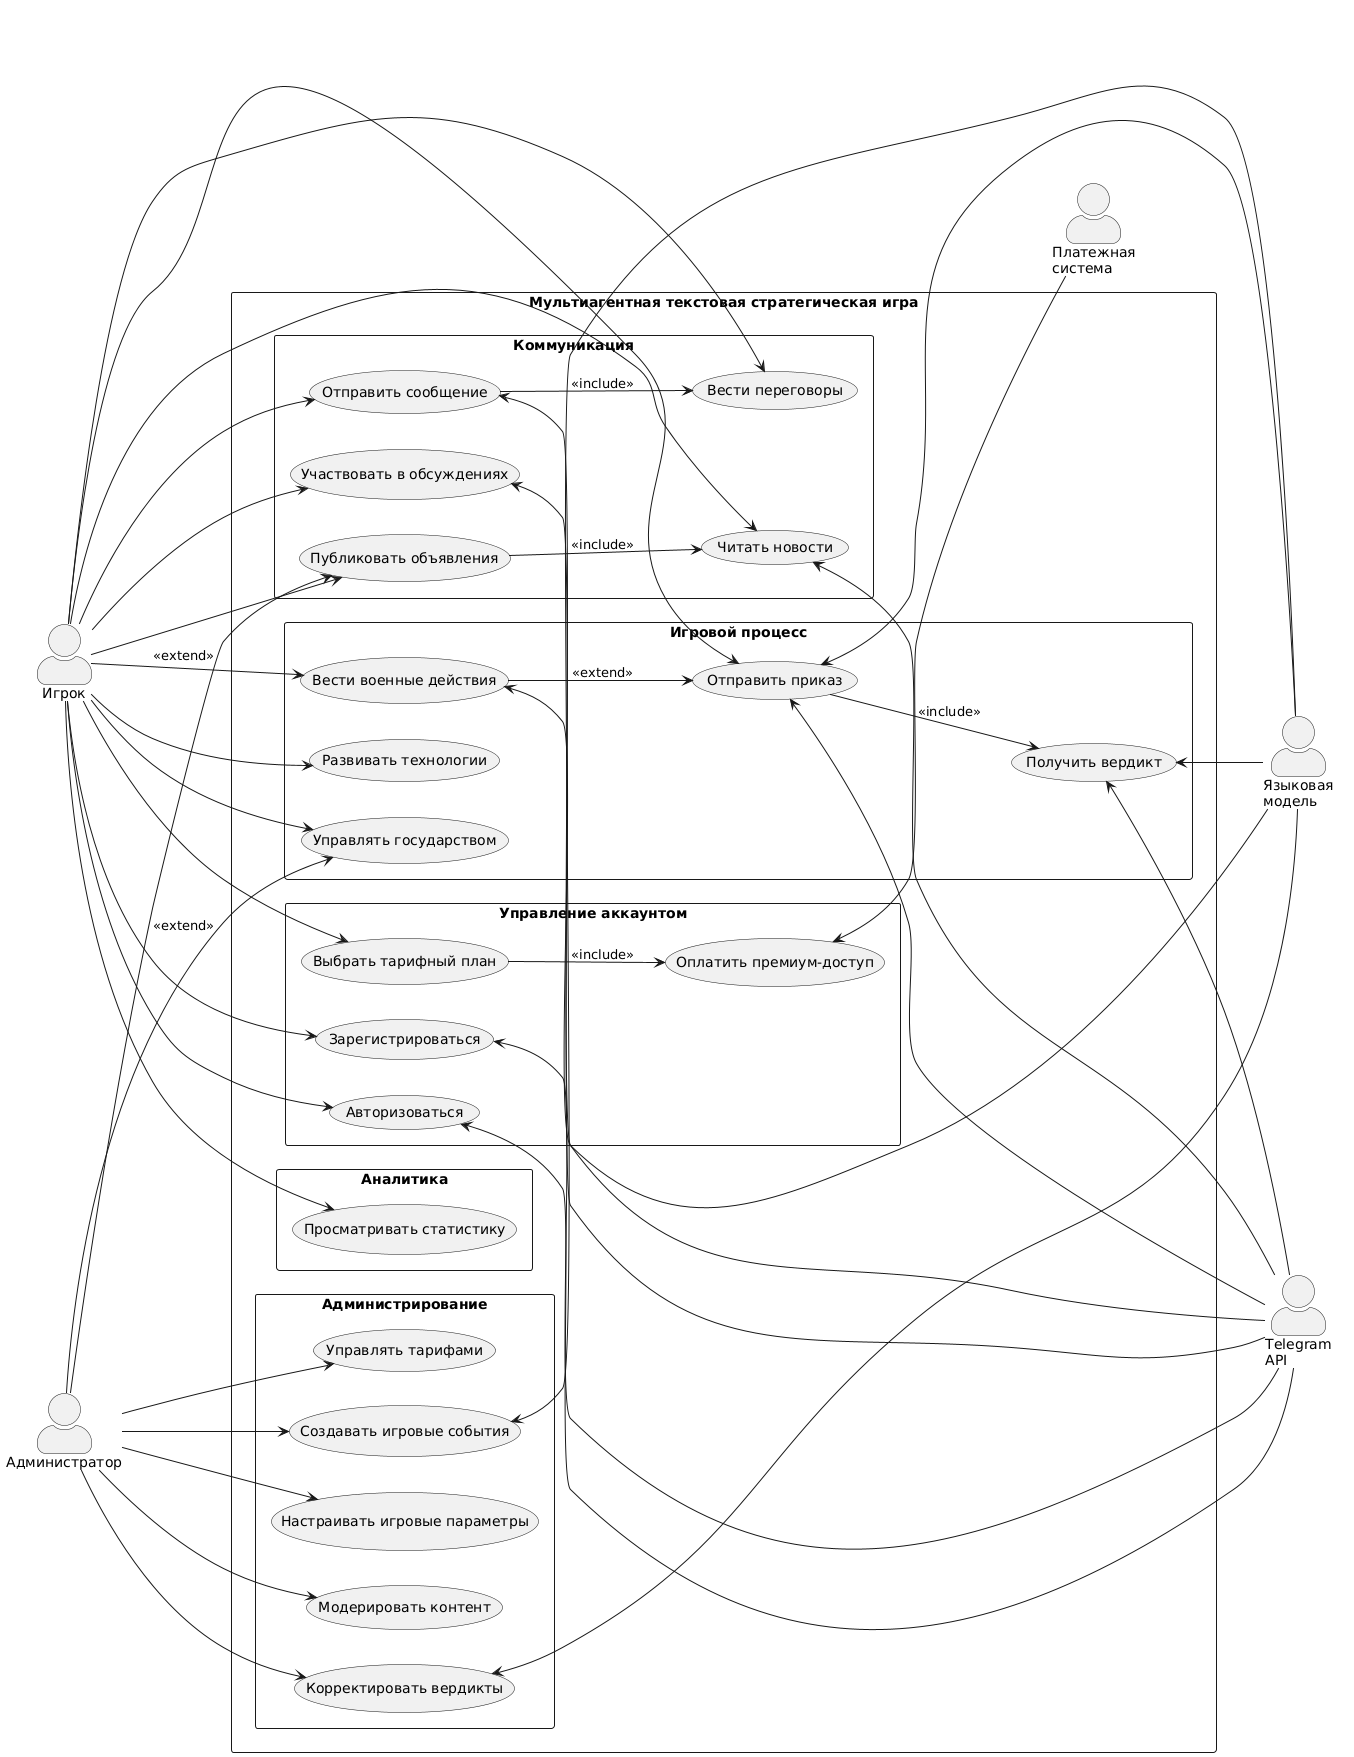
\includegraphics[width=0.7\textwidth]{figures/use-case-diagram.png}
    \caption{Основная диаграмма прецедентов мультиагентной текстовой стратегической игры}
    \label{fig:main-use-case-diagram}
\end{figure}\\
~\\~\\~\\~\\~\\
\newpage
\subsubsection{Ключевые сценарии использования}

Для лучшего понимания функционирования системы ниже представлены детализированные описания ключевых сценариев использования.

\paragraph{UC1: Регистрация нового игрока}

\begin{itemize}
    \item \textbf{Основной актор:} Игрок
    \item \textbf{Предусловия:} Игрок не зарегистрирован в системе
    \item \textbf{Постусловия:} Создан новый аккаунт игрока
    \item \textbf{Основной поток:}
    \begin{enumerate}
        \item Игрок запускает бота в Telegram
        \item Система запрашивает базовую информацию (название ролевого государства, информация о государстве)
        \item Игрок предоставляет запрошенную информацию
        \item Система создает учетную запись и предлагает ознакомиться с обучающими материалами
        \item Игрок просматривает обучающие материалы (опционально)
        \item Система предлагает выбрать тарифный план
        \item Игрок выбирает тарифный план (бесплатный по умолчанию)
        \item Система активирует аккаунт и предоставляет доступ к функциям в соответствии с выбранным тарифом
    \end{enumerate}
    \item \textbf{Альтернативные потоки:}
    \begin{itemize}
        \item Если игрок выбирает платный тарифный план, система перенаправляет его на страницу оплаты
        \item Если никнейм уже занят, система предлагает выбрать другой
        \item Если игрок прерывает процесс регистрации, система сохраняет введенные данные для возможности продолжения позже
    \end{itemize}
\end{itemize}

\paragraph{UC2: Отправка приказа и получение вердикта}

\begin{itemize}
    \item \textbf{Основной актор:} Игрок
    \item \textbf{Предусловия:} Игрок авторизован и имеет активное государство
    \item \textbf{Постусловия:} Приказ обработан, вердикт сгенерирован и доставлен игроку
    \item \textbf{Основной поток:}
    \begin{enumerate}
        \item Игрок формулирует приказ в текстовой форме и отправляет его через интерфейс бота
        \item Система классифицирует тип приказа и проверяет его на соответствие правилам и текущему состоянию игрового мира
        \item Система извлекает релевантный контекст из базы данных (текущее состояние государства, исторические данные, отношения с другими игроками)
        \item Система формирует запрос к языковой модели, включая приказ и контекст
        \item Языковая модель генерирует черновик вердикта
        \item Система проверяет вердикт на согласованность, отсутствие противоречий и соответствие игровым механикам
        \item Система обновляет состояние игрового мира в соответствии с результатами выполнения приказа
        \item Система отправляет окончательный вердикт игроку
        \item Система публикует релевантную информацию в новостной канал, если приказ имеет публичные последствия
    \end{enumerate}
    \item \textbf{Альтернативные потоки:}
    \begin{itemize}
        \item Если приказ нарушает правила игры или технологические ограничения эпохи, система отклоняет его с соответствующим объяснением
        \item Если генерация вердикта требует уточнения деталей приказа, система запрашивает дополнительную информацию у игрока
        \item Если обработка приказа затрагивает другие государства, система учитывает этот факт и генерирует соответствующие уведомления для затронутых игроков
        \item Если система обнаруживает потенциальные противоречия или аномалии в генерируемом вердикте, она сигнализирует об этом администратору для проверки и потенциальной корректировки
    \end{itemize}
\end{itemize}

\paragraph{UC3: Ведение дипломатических переговоров}

\begin{itemize}
    \item \textbf{Основной актор:} Игрок
    \item \textbf{Предусловия:} Игрок авторизован и имеет активное государство
    \item \textbf{Постусловия:} Установлены или модифицированы дипломатические отношения с другим государством
    \item \textbf{Основной поток:}
    \begin{enumerate}
        \item Игрок выбирает опцию "Дипломатия" в интерфейсе бота
        \item Система отображает список других государств с информацией о текущих отношениях
        \item Игрок выбирает государство для установления или изменения дипломатических отношений
        \item Система предлагает варианты действий (отправить сообщение, предложить договор, объявить войну и т.д.)
        \item Игрок выбирает действие и формулирует детали (текст сообщения, условия договора)
        \item Система обрабатывает запрос и доставляет сообщение или предложение выбранному игроку
        \item Получатель принимает решение по поводу предложения
        \item Система обновляет дипломатический статус между государствами в соответствии с принятым решением
        \item Система публикует публичное объявление в новостной канал, если дипломатическое действие имеет публичный характер
    \end{enumerate}
    \item \textbf{Альтернативные потоки:}
    \begin{itemize}
        \item Если получатель отклоняет предложение, система информирует инициатора и сохраняет текущий статус отношений
        \item Если дипломатическое действие требует подтверждения от администратора (например, сложные многосторонние договоры), система направляет запрос на модерацию перед финализацией
        \item Если игрок хочет обсудить детали в свободной форме, система может создать временный зашифрованный канал связи между игроками для проведения переговоров
    \end{itemize}
\end{itemize}

\paragraph{UC4: Управление военными действиями}

\begin{itemize}
    \item \textbf{Основной актор:} Игрок
    \item \textbf{Предусловия:} Игрок находится в состоянии войны с другим государством
    \item \textbf{Постусловия:} Военные действия разрешены с определенным исходом
    \item \textbf{Основной поток:}
    \begin{enumerate}
        \item Игрок формулирует военный приказ, включающий цели, используемые войска и тактические указания
        \item Система проверяет легитимность приказа (наличие объявленной войны, доступность указанных войск)
        \item Система определяет, затрагивает ли приказ другие государства, и если да, запрашивает их ответные действия
        \item Система собирает все релевантные военные приказы и формирует полный контекст сражения
        \item Система активирует военный режим, позволяющий более динамичную обработку приказов во время боя
        \item Система формирует запрос к языковой модели для симуляции сражения
        \item Языковая модель генерирует описание хода сражения и его результатов
        \item Система определяет количественные последствия сражения (потери, захваченные территории)
        \item Система отправляет детальные вердикты всем участникам конфликта
        \item Система публикует публичное описание сражения в новостной канал
        \item Система обновляет состояние игрового мира в соответствии с результатами сражения
    \end{enumerate}
    \item \textbf{Альтернативные потоки:}
    \begin{itemize}
        \item Если приказы сторон требуют уточнения, система запрашивает дополнительную информацию перед симуляцией
        \item Если результаты симуляции кажутся неправдоподобными, система может запросить ручную проверку администратором
        \item Если военные действия включают особо сложные или масштабные операции, система может задействовать специализированные алгоритмы симуляции боя вместо прямой генерации текста
    \end{itemize}
\end{itemize}

\paragraph{UC5: Модерация и корректировка вердиктов}

\begin{itemize}
    \item \textbf{Основной актор:} Администратор
    \item \textbf{Предусловия:} Система идентифицировала потенциальные проблемы в генерируемом вердикте или получила апелляцию от игрока
    \item \textbf{Постусловия:} Вердикт скорректирован или подтвержден
    \item \textbf{Основной поток:}
    \begin{enumerate}
        \item Система уведомляет администратора о потенциальной проблеме в вердикте
        \item Администратор просматривает исходный приказ, контекст и сгенерированный вердикт
        \item Администратор принимает решение о необходимости корректировки
        \item Если корректировка необходима, администратор вносит изменения в вердикт
        \item Система обновляет состояние игрового мира в соответствии с скорректированным вердиктом
        \item Система отправляет окончательный вердикт игроку с пометкой о модерации
        \item Система регистрирует факт модерации для аналитики и обучения
    \end{enumerate}
    \item \textbf{Альтернативные потоки:}
    \begin{itemize}
        \item Если администратор подтверждает корректность исходного вердикта, система информирует игрока о результатах рассмотрения апелляции
        \item Если проблема указывает на систематическую ошибку в работе языковой модели, администратор может внести изменения в параметры системы или промпты для предотвращения подобных проблем в будущем
    \end{itemize}
\end{itemize}

\paragraph{UC6: Чтение новостей и участие в обсуждениях}

\begin{itemize}
    \item \textbf{Основной актор:} Игрок
    \item \textbf{Предусловия:} Игрок подписан на новостной канал и имеет доступ к общему чату
    \item \textbf{Постусловия:} Игрок получил информацию о событиях в игровом мире и участвовал в обсуждении
    \item \textbf{Основной поток:}
    \begin{enumerate}
        \item Система публикует новостное сообщение в канал (автоматически или по решению администратора)
        \item Игрок получает уведомление и просматривает новость
        \item Игрок переходит в связанный чат для обсуждения новости
        \item Игрок участвует в обсуждении, публикуя сообщения и отвечая другим участникам
        \item Система мониторит обсуждение на предмет нарушения правил коммуникации
        \item Игрок получает уведомления о новых ответах на его сообщения
        \item Игрок может запросить дополнительную информацию о событии через интерфейс бота
    \end{enumerate}
    \item \textbf{Альтернативные потоки:}
    \begin{itemize}
        \item Если система обнаруживает нарушение правил в сообщениях игрока, она предупреждает его или скрывает спорный контент
        \item Если обсуждение затрагивает личные дипломатические вопросы, игроки могут перейти в приватную беседу для продолжения переговоров
        \item Если новость вызывает значительный резонанс, администратор может организовать специальное мероприятие или опрос для дальнейшего развития сюжета
    \end{itemize}
\end{itemize}

\paragraph{UC7: Взаимодействие с мультиагентной системой (внутренний сценарий)}

\begin{itemize}
    \item \textbf{Основные акторы:} Языковая модель, компоненты мультиагентной системы
    \item \textbf{Предусловия:} Получен приказ игрока, требующий обработки
    \item \textbf{Постусловия:} Сгенерирован вердикт, согласованный между всеми агентами
    \item \textbf{Основной поток:}
    \begin{enumerate}
        \item Агент-классификатор определяет тип и сферу действия приказа
        \item Агент-валидатор проверяет соответствие приказа правилам и ограничениям игрового мира
        \item Агент-извлечения контекста собирает релевантную информацию из базы данных
        \item Агент-экономист оценивает экономические последствия приказа
        \item Агент-дипломат определяет потенциальное влияние на межгосударственные отношения
        \item Агент-стратег (при необходимости) моделирует военные последствия
        \item Агент-координатор интегрирует результаты анализа от всех агентов
        \item Агент-генератор формирует запрос к языковой модели на основе обработанных данных
        \item Языковая модель генерирует текст вердикта
        \item Агент-валидатор проверяет вердикт на согласованность и отсутствие противоречий
        \item Агент-координатор финализирует вердикт и передает его для доставки игроку
        \item Агент-архивариус обновляет состояние игрового мира и историческую базу данных
    \end{enumerate}
    \item \textbf{Альтернативные потоки:}
    \begin{itemize}
        \item Если обнаружены противоречия между оценками разных агентов, агент-координатор инициирует процедуру согласования
        \item Если приказ признан невалидным на любом этапе, процесс прерывается и игроку отправляется соответствующее уведомление
        \item Если генерация вердикта требует вмешательства человека, агент-координатор эскалирует задачу администратору
    \end{itemize}
\end{itemize}

Представленные диаграммы прецедентов и сценарии использования обеспечивают общее понимание функциональности системы и взаимодействия пользователей с ней. Они служат основой для проектирования архитектуры системы и разработки конкретных компонентов, соответствующих выявленным требованиям.

\subsection{Требования к пользовательскому интерфейсу}

Пользовательский интерфейс играет критическую роль в обеспечении доступности и удобства игрового процесса. Учитывая, что основной платформой для взаимодействия с игрой выбран Telegram, разработка интерфейса должна максимально эффективно использовать возможности этой платформы при одновременном сохранении естественного диалогового формата, характерного для жанра ВПИ.

\subsubsection{Общие принципы проектирования интерфейса}

При разработке пользовательского интерфейса следует руководствоваться следующими принципами:

\begin{itemize}
    \item \textbf{Естественность диалога} — интерфейс должен обеспечивать максимально естественное текстовое взаимодействие, минимизируя необходимость использования специальных команд или форматирования.

    \item \textbf{Минимализм и ненавязчивость} — элементы интерфейса не должны отвлекать от основного текстового взаимодействия, а служить вспомогательными инструментами, доступными по запросу.

    \item \textbf{Информативность} — игроки должны получать чёткую и своевременную обратную связь о результатах своих действий и текущем состоянии игры.

    \item \textbf{Контекстуальность} — система должна сохранять и учитывать контекст диалога, обеспечивая согласованность взаимодействия.

    \item \textbf{Соответствие стилистике игры} — визуальные элементы и тон коммуникации должны соответствовать жанру и сеттингу игры, повышая уровень погружения.

    \item \textbf{Доступность} — интерфейс должен быть интуитивно понятен пользователям с различными уровнями технической подготовки и на различных устройствах.
\end{itemize}

\subsubsection{Структура интерфейса в Telegram}

Интерфейс игры в Telegram должен включать следующие ключевые компоненты:

\paragraph{Основной игровой бот}

\begin{itemize}
    \item \textbf{Диалоговый интерфейс} — основной способ взаимодействия с игрой через свободный текстовый диалог, где игрок может формулировать приказы, задавать вопросы и инициировать действия в естественной форме.

    \item \textbf{Стартовый экран} с приветствием и основной информацией об игре для новых пользователей, кратким объяснением принципов взаимодействия и примерами возможных действий.

    \item \textbf{Информационные команды} — минимальный набор специальных команд для получения справочной информации (например, /help, /status, /info), доступных через меню бота, но не обязательных для использования.

    \item \textbf{Система уведомлений} о значимых событиях, получении вердиктов и действиях других игроков, затрагивающих интересы пользователя.

    \item \textbf{Контекстуальные подсказки} — ненавязчивые рекомендации возможных действий в зависимости от текущей ситуации, предлагаемые в моменты паузы в диалоге или при запросе помощи.
\end{itemize}

\paragraph{Новостной канал}

\begin{itemize}
    \item \textbf{Структурированная лента новостей} с чётким разделением на глобальные события, региональные новости и информацию о конкретных государствах.

    \item \textbf{Система тегов} для визуальной категоризации новостей (дипломатия, военные конфликты, экономика, исследования, культура) с помощью эмодзи и цветового кодирования.

    \item \textbf{Перекрестные ссылки} между взаимосвязанными новостями для обеспечения целостного понимания развития событий.

    \item \textbf{Визуальное оформление} новостных сообщений с использованием форматирования текста, эмодзи и, при необходимости, иллюстраций.
\end{itemize}

\paragraph{Обсуждения и коммуникация}

\begin{itemize}
    \item \textbf{Общий чат} для обсуждения игровых событий и взаимодействия между участниками.

    \item \textbf{Тематические обсуждения}, привязанные к конкретным новостям или событиям.

    \item \textbf{Интеграция с дипломатической системой} — возможность инициировать официальные переговоры с другими государствами непосредственно из чата с сохранением результатов в игровом контексте.

    \item \textbf{Формат ролевого общения} с поддержкой официальной коммуникации от имени государства и неформального общения от имени игрока.
\end{itemize}

\subsubsection{Требования к диалоговому взаимодействию}

Учитывая специфику диалогового формата, особое внимание следует уделить следующим аспектам:

\begin{itemize}
    \item \textbf{Естественное языковое понимание} — система должна корректно интерпретировать приказы и вопросы, сформулированные в свободной форме, без необходимости использования специального синтаксиса или ключевых слов.

    \item \textbf{Контекстуальная память} — система должна сохранять контекст диалога, позволяя игрокам ссылаться на предыдущие сообщения или обсуждаемые объекты без необходимости явного повторения ключевой информации.

    \item \textbf{Интеллектуальная классификация} — система должна автоматически определять тип сообщения (приказ, вопрос, проект, обсуждение) и реагировать соответствующим образом без необходимости явного указания типа действия.

    \item \textbf{Подтверждение понимания} — в случаях, когда запрос неоднозначен или требует уточнения, система должна запрашивать дополнительную информацию или предлагать свое понимание на подтверждение перед выполнением действия.

    \item \textbf{Адаптивный стиль коммуникации} — система должна адаптировать стиль ответов под особенности коммуникации конкретного игрока, поддерживая последовательность в формальном/неформальном тоне, детализации и структуре сообщений.
\end{itemize}

\subsubsection{Требования к текстовому представлению информации}

Текстовое представление является основным способом передачи информации в игре, поэтому важно обеспечить его эффективность:

\begin{itemize}
    \item \textbf{Чёткое форматирование текста} с использованием возможностей Markdown для выделения заголовков, важной информации, цитат и т.д.

    \item \textbf{Структурированное представление вердиктов} с логическим разделением на вводную часть, описание процесса, результаты и последствия.

    \item \textbf{Информационная иерархия} — важнейшая информация должна располагаться в начале сообщения, с постепенным переходом к детализации и контекстуальным данным.

    \item \textbf{Дозированная подача информации} — разбиение длинных текстов на логические блоки с возможностью последовательного просмотра для избежания перегрузки чата.

    \item \textbf{Емкость и выразительность} — использование богатого языка для создания атмосферы при сохранении информативности и лаконичности сообщений.
\end{itemize}

\subsubsection{Требования к визуальным элементам}

Несмотря на преимущественно текстовый характер игры, визуальные элементы могут значительно обогатить игровой опыт:

\begin{itemize}
    \item \textbf{Интерактивная карта мира} — предоставляемая по запросу ("покажи карту", "какие территории контролирует Инферия") с возможностью фокусировки на конкретных регионах.

    \item \textbf{Экономические и статистические графики}, генерируемые по запросу для анализа динамики развития государства.

    \item \textbf{Иконки и эмодзи} для быстрой визуальной идентификации типов сообщений, статусов и категорий информации.

    \item \textbf{Генерируемые изображения} для иллюстрации ключевых событий и результатов действий (опционально, в зависимости от выбранного тарифа).

    \item \textbf{Визуальная индикация статуса} государств (мирное время/война, экономический рост/кризис) через цветовое кодирование или специальные маркеры в информационных сводках.
\end{itemize}

\subsubsection{Требования к эргономике и удобству использования}

\begin{itemize}
    \item \textbf{Предсказуемые ответы} — система должна обеспечивать последовательность и предсказуемость в реакциях на сходные запросы и действия.

    \item \textbf{Экономия действий пользователя} — минимизация необходимых действий для достижения цели, особенно для часто повторяющихся операций.

    \item \textbf{Информативная обратная связь} — система должна явно подтверждать получение и обработку запросов, особенно если формирование ответа требует времени.

    \item \textbf{Обработка ошибок} — в случае непонимания запроса система должна предлагать альтернативные формулировки или уточняющие вопросы, а не просто сообщать о невозможности выполнения.

    \item \textbf{История взаимодействия} с возможностью быстрого доступа к предыдущим приказам и вердиктам (например, через команду "покажи мои последние приказы" или "что я делал вчера").

    \item \textbf{Контекстуальная помощь} — возможность в любой момент запросить рекомендации по формулировке приказов или использованию системы в контексте текущей ситуации.
\end{itemize}

\subsubsection{Требования к адаптивности и доступности}

\begin{itemize}
    \item \textbf{Корректное отображение} на различных устройствах (смартфоны, планшеты, десктопы) и в различных клиентах Telegram.

    \item \textbf{Оптимизация для мобильного использования} с учетом особенностей взаимодействия на сенсорных экранах.

    \item \textbf{Поддержка голосового ввода} для приказов с возможностью автоматической транскрипции голосовых сообщений в текст.

    \item \textbf{Настройки форматирования текста} для пользователей с особыми потребностями (увеличенный размер шрифта, высокий контраст).

    \item \textbf{Локализация интерфейса} с поддержкой русского и английского языков (на начальном этапе).
\end{itemize}

\subsubsection{Примеры ключевых взаимодействий}

\paragraph{Приветствие нового игрока}

\begin{verbatim}
👋 Добро пожаловать в RELOAD WPG!

Я — ИИ-ассистент, который поможет вам управлять вашим государством в
текстовой стратегической игре Reload. Вы можете общаться со мной на
естественном языке — задавать вопросы, отдавать приказы и планировать проекты.

🌍 Для начала, давайте создадим ваше государство:
• Какое название вы хотели бы дать своей стране?
• Каким будет государственный строй?
• Какие особенности и ценности важны для вашего народа?

Просто ответьте на эти вопросы в свободной форме, и мы начнем наше путешествие.

💡 В любой момент вы можете спросить меня "Что я могу сделать?" или
"Помоги мне", и я предложу возможные действия.
\end{verbatim}

\paragraph{Диалог с игроком}

\begin{verbatim}
Игрок: Какое текущее состояние нашей экономики?

🔍 Экономический анализ Республики Лурк
====================
📅 Дата: 1 января 2200 года

📊 Основные показатели:
• ВВП: 1.2 трлн кредитов (рост +2.3% за квартал)
• Инфляция: 1.7% (стабильная)
• Безработица: 4.8% (снижение на 0.2%)
• Государственный долг: 15% от ВВП

💰 Состояние бюджета:
• Доходы: 305 млрд кредитов
• Расходы: 298 млрд кредитов
• Профицит: 7 млрд кредитов (0.6% ВВП)

🏭 Ключевые отрасли:
• Космическая промышленность — динамичный рост (+8.5%)
• Энергетика — стабильное состояние (+1.2%)
• Сельское хозяйство — умеренный рост (+3.7%)
• Тяжелая промышленность — стагнация (-0.3%)

⚠️ Проблемные зоны:
• Зависимость от импорта редкоземельных металлов
• Устаревающая транспортная инфраструктура в восточных регионах
• Растущее неравенство между столицей и периферией

📈 [Посмотреть подробные графики и отчеты]
====================

Игрок: Хочу начать программу модернизации транспортной сети в восточных
провинциях. Выделим 150 миллионов кредитов на первый этап, сосредоточимся
на создании высокоскоростных магистралей между ключевыми
промышленными центрами.

✅ Приказ принят
====================
Министерство инфраструктуры приступает к реализации программы модернизации
транспортной сети в восточных провинциях.

Я проанализировал ситуацию и рассчитываю, что первый этап займет примерно 8
месяцев. Текущее финансирование в 150 млн кредитов позволит модернизировать
около 35% ключевых магистралей, соединяющих промышленные центры региона.

Проект "Восточный транспортный коридор" добавлен в список активных проектов.
Первые результаты ожидаются через 2 месяца.

⏱️ Желаете ускорить реализацию проекта или оставить текущий темп?
====================

Игрок: Текущий темп меня устраивает. Давай также увеличим инвестиции в
исследование альтернативных источников редкоземельных металлов. Нам
нужно снизить импортную зависимость.

✅ Приказ принят
====================
Министерство науки и технологий запускает исследовательскую программу по
разработке альтернативных источников редкоземельных металлов и технологий
их замещения.

На основе анализа текущего бюджета на НИОКР, рекомендую выделить на эту
программу 85 млн кредитов в год. Этого будет достаточно для финансирования
3-4 перспективных направлений исследований.

🔍 Наиболее перспективные направления:
• Разработка месторождений на континентальном шельфе
• Создание композитных материалов с аналогичными свойствами
• Переработка электронных отходов для извлечения редкоземельных элементов
• Синтез искусственных аналогов

Проект "Ресурсная независимость" добавлен в список активных проектов.
Первые научные результаты ожидаются через 4-6 месяцев, практические
прототипы — не ранее чем через 14 месяцев.

📊 Расчетное снижение импортной зависимости: до 15% в течение 3 лет.
====================
\end{verbatim}

\paragraph{Получение информации о мире}

\begin{verbatim}
Игрок: Расскажи о наших отношениях с Империей Хуан-Фернандес. Какие у них
сильные и слабые стороны?

🌐 Империя Хуан-Фернандес: дипломатический профиль
====================
📅 Актуально на: 1 января 2200 года

🤝 Текущие отношения с Республикой Лурк:
• Официальный статус: Напряженный нейтралитет
• Торговые отношения: Ограниченная торговля (объем 45.2 млрд кредитов в год)
• Дипломатические инциденты: Пограничный спор в секторе Альфа-9 (не разрешен)
• Культурный обмен: Минимальный

💪 Сильные стороны:
• Мощный военно-космический флот (крупнейший в известном космосе)
• Передовые технологии в области квантовой связи
• Устойчивая ресурсная база благодаря контролю над системой Проксима
• Централизованная эффективная система управления

🔍 Уязвимости:
• Растущее внутреннее сопротивление имперской политике
• Экономическая стагнация в колониальных секторах
• Чрезмерная милитаризация истощает гражданскую экономику
• Напряженные отношения с Федерацией Инферии, отвлекающие ресурсы

⚠️ Потенциальные точки конфликта:
• Экспансия в нейтральные системы на границе с Лурком
• Конкуренция за редкоземельные ресурсы
• Идеологические противоречия (империализм vs республиканизм)

💡 Возможности для сотрудничества:
• Совместные исследования в области экзопланетологии
• Создание буферной зоны для снижения напряженности
• Расширение культурного обмена для улучшения взаимопонимания

📜 [Доступ к полной истории взаимоотношений]
====================
\end{verbatim}

\subsubsection{Заключение}

Пользовательский интерфейс мультиагентной текстовой стратегической игры должен быть сфокусирован на обеспечении естественного диалогового взаимодействия с игроком, минимизируя барьеры входа и технические сложности. Ключевым принципом является интеллектуальное понимание намерений игрока вне зависимости от формулировки, что позволяет сохранить свободу творческого самовыражения и аутентичность жанра ВПИ.

Telegram как платформа предоставляет необходимый инструментарий для реализации такого подхода, включая поддержку форматированного текста, мультимедиа и организации коммуникационных каналов между игроками. Важно, чтобы интерфейс оставался ненавязчивым, выдвигая на первый план содержательные аспекты игры и взаимодействие между участниками, а не технические механики.

Разработанный с учетом этих требований интерфейс позволит игрокам с различным уровнем подготовки и предпочтений комфортно погрузиться в игровой мир, фокусируясь на принятии стратегических решений, дипломатии и социальном взаимодействии, а не на изучении сложных игровых систем.

\subsection{Стратегия обработки ошибок и исключительных ситуаций}

\subsection{Масштабируемость и производительность}

\subsection{Этические аспекты и ограничения системы}